\newpage
\titleformat{\section}[block] % change setting for basic sections
{\bfseries\normalsize}{\thesection}{1em}{}
\titlespacing\section{\parindent}{\parskip}{\parskip} 

\section{Кавитация}
\subsection{Введение}
\vspace{0.5\baselineskip}

Кавитация — это процесс образования и последующего коллапса паровых пузырей в жидкости, который обычно возникает из-за резких изменений давления.
При коллапсе этих пузырей образуются высокоскоростные струи и ударные волны, что приводит к локальному изменению таких параметров, как распределение скоростей, давление, плотность, температура, энергия и других в области коллапса~\cite{10.2478/s11534-009-0092-y}.
Кавитация приводит к образованию паровых полостей в изначально однородной жидкой среде и может проявляться в различных ситуациях в зависимости от физических свойств жидкости и конфигурации потока.
Кавитация возникает вследствие локального нарушения сплошности жидкой среды при достижении очень низких давлений, что делает её важным явлением в механике сплошных сред и применимой как к неподвижным, так и к движущимся жидкостям.

Пороговое давление, ниже которого жидкость теряет свою когезию, является одним из ключевых параметром кавитации.
Хотя этот порог определяется параметрами жидкости и среды и должен определяться на микроскопическом уровне, для практических применений приходится ориентироваться на макроскопические свойства жидкости.
Например, при заполнении шприца медленным движением поршня поддерживается достаточно высокое давление внутри шприца, чтобы избежать разрыва жидкости.
При быстром движении поршня статическое давление в игле падает, что может вызвать образование полостей и прекращение заполнения. 
Дополнительные турбулентные флуктуации давления в шприце также способствуют снижению локального давления до уровня насыщенного пара, что приводит к образованию пара и прекращению заполнения.
Подобное явление также встречается в объёмных насосах, например, в системах подачи топлива в двигатели, где потери давления и резкое ускорение жидкостного столба могут привести к понижению давления и, следовательно, к кавитации.

С точки зрения классической термодинамики, кавитацию можно рассматривать как процесс, аналогичный кипению, но с изменением давления вместо изменения температуры.
На фазовой диаграмме воды кривая от тройной точки до критической точки разделяет области жидкости и пара, и переход через эту кривую представляет собой обратимый процесс при равновесных условиях.
Кавитация происходит, когда давление в жидкости снижается до уровня ниже давления насыщенного пара при почти постоянной температуре, что чаще всего наблюдается в реальных течениях, где изменение давления контролируется динамикой потока~\cite{10.1007/1-4020-2233-6}.


\begin{figure}[h] % [h] place the float here, i.e., approximately at the same point it occurs in the source text (however, not exactly at the spot)
    \centering
    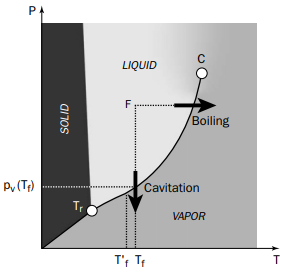
\includegraphics[height=.3\textheight]{images/phase_diagram.png}
    \caption{\centering  Фазовая диаграмма~\cite{10.1007/1-4020-2233-6}}
    \label{fig:phase_diagram}
\end{figure}

В большинстве случаев возникновения кавитации, особенно при использовании холодной воды, для образования значительного объёма пара требуется лишь относительно небольшое количество тепла, что приводит к минимальному изменению температуры окружающей жидкости.
Таким образом, процесс испарения на фазовой диаграмме можно считать практически изотермичным (рисунок~\ref{fig:phase_diagram}).
Однако в некоторых случаях передача тепла, необходимая для кавитационного испарения, происходит таким образом, что фазовый переход происходит при температуре \( T' \), которая ниже температуры окружающей жидкости \( T \).
Разность температур \( T - T' \) называется тепловым запаздыванием в кавитации, и она возрастает, когда температура окружающей среды приближается к критической температуре жидкости. Это явление имеет важное значение, например, при перекачке криогенных жидкостей в ракетных двигателях.

С теоретической точки зрения можно выделить несколько этапов, которые происходят в первые моменты кавитации:
\begin{itemize}
  \item разрушение или образование пустоты;
  \item заполнение пустоты паром;
  \item возможное насыщение пустоты паром.
\end{itemize}

На практике эти этапы протекают практически одновременно, при этом второй этап происходит настолько быстро, что его можно считать мгновенным, а пустоту — сразу насыщенной паром. Следует отметить, что кривая \( p_v(T) \) не является абсолютной границей между состояниями жидкости и пара. Отклонения от этой кривой возможны в случае быстрого фазового перехода.

\begin{figure}[h]
    \centering
    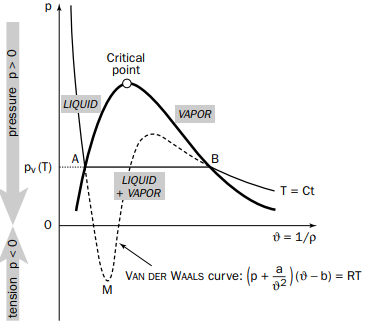
\includegraphics[height=.3\textheight]{images/isotherms.png}
    \caption{\centering  Изотермы Эндрюса (сплошная линия) и Ван-дер-Ваальса (пунктирная линия)~\cite{10.1007/1-4020-2233-6}}
    \label{fig:isotherms}
\end{figure}

Даже при почти статичных условиях фазовый переход может происходить при давлении, меньшем, чем парциальное давление \( p_v \). 
Рассмотрим, например, так называемые изотермы Эндрюса на диаграмме \( p \) — \( V \), где \( V = \frac{1}{\rho} \) — удельный объём, а \( \rho \) — плотность (рисунок~\ref{fig:isotherms}).
Эти кривые могут быть аппроксимированы с помощью уравнения состояния Ван дер Ваальса для жидкой и паровой фаз.
Переход из жидкости в пар вдоль пути \( AM \) можно предотвратить, если в ходе эксперимента будут соблюдены определённые осторожные меры.
Вдоль этого пути жидкость остаётся в метастабильном состоянии и может даже выдерживать отрицательные абсолютные давления, то есть напряжения, без перехода в другую фазу.
Таким образом, условие, при котором локальное абсолютное давление равно парциальному давлению при температуре всей системы, не всегда является достаточным для начала кавитации.
Разница между парциальным давлением и фактическим давлением, при котором возникает кавитация, называется статическим запаздыванием.
В некоторых случаях также наблюдается динамическое запаздывание, обусловленное инерционными эффектами, связанными с временем, необходимым для того, чтобы паровые полости стали видимыми.

Кавитация может проявляться в различных формах на различных стадиях своего развития, начиная с момента возникновения. 
Изначально её развитие в значительной степени зависит от основного потока, не вызывающего кавитацию. 
Однако по мере роста паровых структур они начинают нарушать и изменять характер потока. В
зависимости от стадии и условий кавитации можно выделить следующие основные формы кавитационных пузырей~\cite{10.1007/1-4020-2233-6}:

\begin{itemize} 
    \item Преходящие изолированные пузырьки. Эти пузырьки возникают в области низкого давления в результате быстрого роста очень мелких воздушных ядер -- микроскопических пузырьков, возникающих в жидкости в результате предыдущих процессов (например, растворённый воздух), микронеровностей на стенках сосудов, частиц загрязнений или флуктуаций. Такие пузырьки переносятся основным потоком и исчезают, когда попадают в области с достаточно высоким давлением.
    \item Прикрепленные или пленочные полости. Данные полости часто фиксируются на переднем крае тела, например, на стороне низкого давления лопаток и крыльев, где они образуют стабильные структуры.
    \item Кавитирующие вихри. Вихри, возникающие в области низкого давления, могут служить ядром для формирования кавитации. Она может проявляться в турбулентных следах вихрей или как регулярный узор в вихрях на концах трехмерных крыльев или лопаток винтов. Некоторые формы кавитации трудно отнести к одной из перечисленных категорий. Например, на низкодавление поверхностях крыльев или лопаток винтов могут возникать паровые структуры с очень коротким временем существования, которые имеют форму прикрепленных полостей, но ведут себя как движущиеся пузырьки.  
\end{itemize}

Одними из важнейших работ, позволяющих дать количественную оценку кавитации и объясняющих природу этого явления являются работы Харуми~\cite{http://dx.doi.org/10.1121/1.409850} и Немчевски~\cite{10.1016/0041-624x(80)90021-9}, в которых на основе теории флуктуаций, предложенной Ландау и Лифшицем~\cite{landau1980statistical}, было доказано, что кавитация может возникать как за счет объемных флуктуаций, так и за счет флуктуаций пузырьков пара. Этот вывод был сделан на основе взаимосвязи между прочностью жидкости на разрыв и объемными флуктуациями. Полученная вероятность кавитации выражается через вероятности обоих типов флуктуаций, что подчеркивает важную роль флуктуаций в жидкостях в реальных кавитационных процессах.

Чаще всего кавитацию наблюдают в промышленном оборудовании, таком как насосы и турбины, где пузырьковый коллапс вызывает эрозию и снижает эффективность системы~\cite{10.1016/j.rser.2009.07.024}.
Кавитационный пузырь вблизи жесткой поверхности демонстрирует сложную несимметричную динамику, изображенную на рисунке~\ref{fig:cavitation_damage}.
Пузырь достигает своего максимального размера (1). 
Из-за близости твердой поверхности, создающей граничное условие для скорости на нижней границе, его верхняя граница схлопывается быстрее, чем часть, расположенная ближе к стенке (2 и 3). Формируется микроструя (3), скорость которой может достигать нескольких сотен м/с.
При ударе микроструи о твердую поверхность возникает ударное давление (уравнение (2)), достаточное для деформации поверхности (4). После схлопывания, вызванного микроструей, поток жидкости движется радиально наружу (5), вызывая вторичное испарение или ''разбрызгивание''~\cite{10.1017/s0022112071001058} (6).
Это приводит к образованию множества микроскопических пузырьков (размером в микрометры), которые благодаря силам поверхностного натяжения сохраняют сферическую форму при схлопывании. В результате формируются локальные пики давления и мощные ударные волны (7), способные снова вызвать деформацию материала.

\begin{figure}[h] % [h] place the float here, i.e., approximately at the same point it occurs in the source text (however, not exactly at the spot)
    \centering
    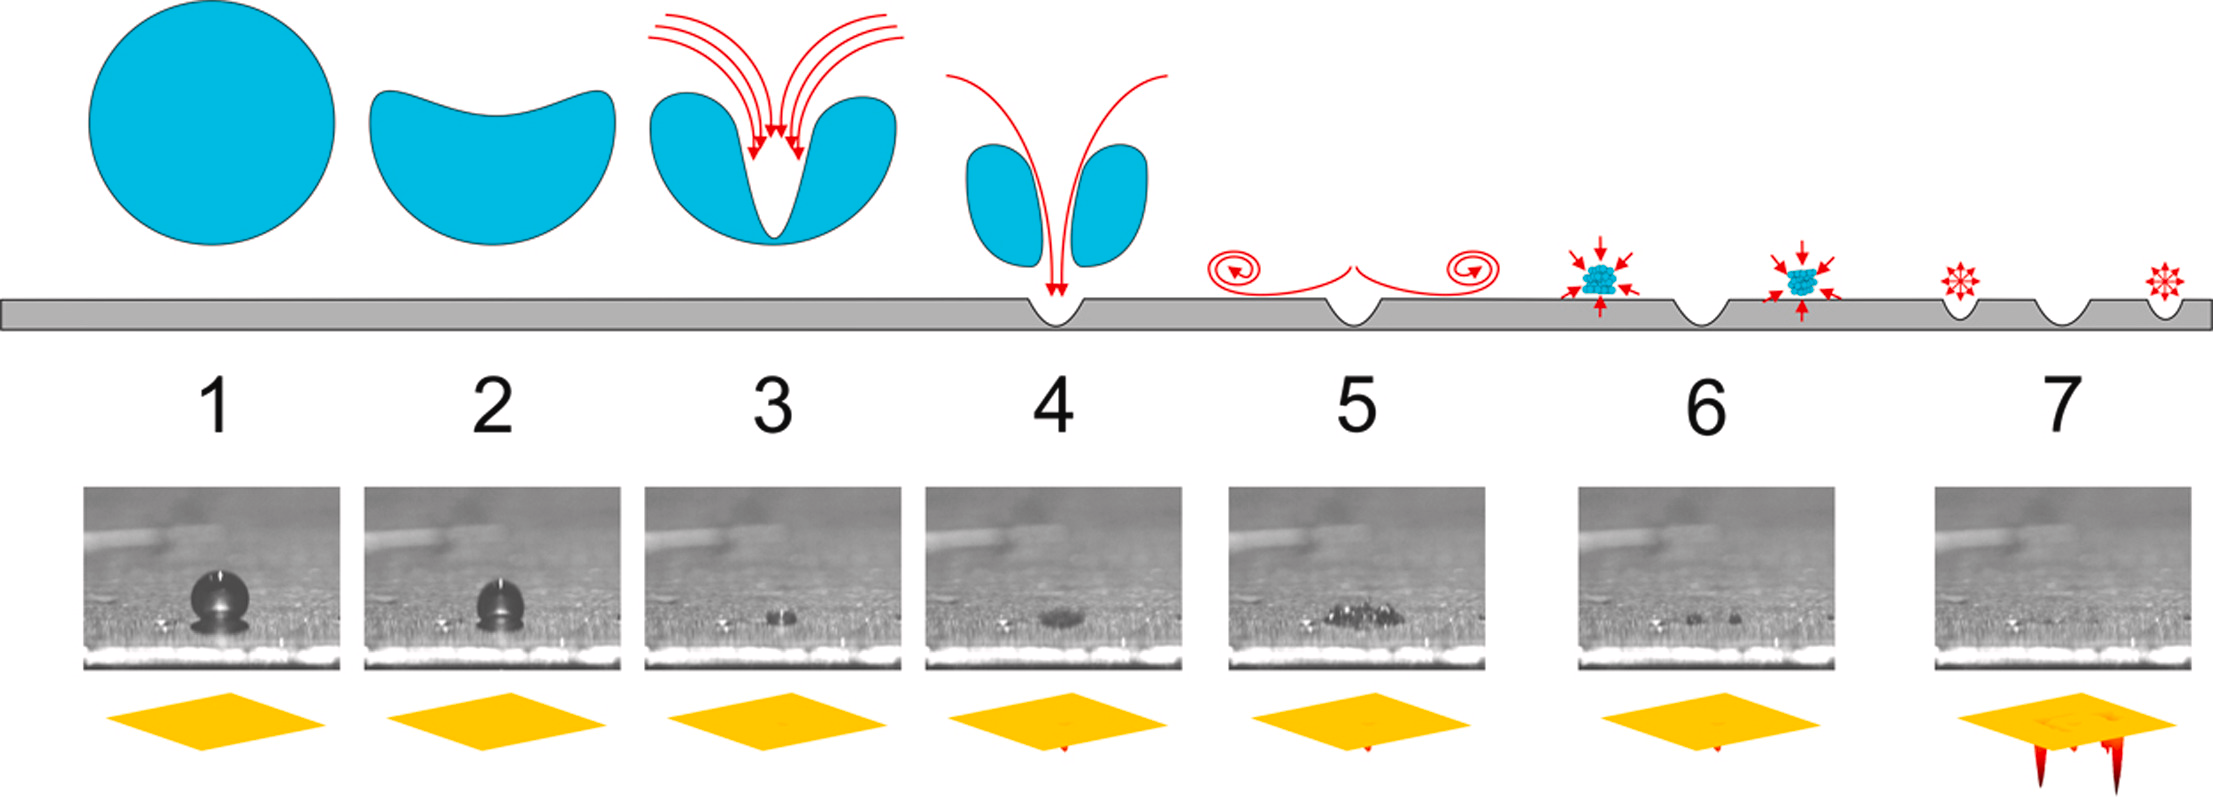
\includegraphics[width=\textwidth]{images/cavitation_damage.png}
    \caption{\centering Два возможных механизма возникновения кавитационной эрозии~\cite{10.1016/j.wear.2018.11.004}}
    \label{fig:cavitation_damage}
\end{figure}

%Однако кавитация не только разрушительный процесс, она также находит множество полезных применений в различных областях.
%В медицине кавитация используется в передовых технологиях, например, при неинвазивных операциях на глазах, точечной доставке лекарств и разрушении камней в почках~\cite{10.1098/rsfs.2015.0022}.
%В промышленности кавитация применяется в ультразвуковой очистке и обработке материалов, а также для повышения эффективности морских винтов и гидравлических турбин~\cite{10.1016/j.scitotenv.2020.139606, 10.3390/met10020270}.
%Также кавитация проявляется в широком спектре форм, каждая из которых обусловлена особенностями окружающей среды и методами её инициирования.
%Это разнообразие условий возникновения определяет значимость кавитации для изучения в различных областях науки и техники, включая гидродинамику, медицинскую акустику и лазерные технологии.

Однако кавитация представляет собой не только разрушительное явление, но и мощный инструмент, нашедший широкое практическое применение в различных сферах.
В медицинской сфере кавитационные технологии используются в проведении неинвазивных офтальмологических операций, таргетированной доставке фармацевтических препаратов, экстракорпоральной литотрипсии (дробление почечных конкрементов)~\cite{10.1098/rsfs.2015.0022}.
В промышленном производстве кавитация успешно применяется для прецизионной ультразвуковой очистки сложных поверхностей, модификации свойств конструкционных материалов, оптимизации гидродинамических характеристик судовых двигателей и турбинных установок~\cite{10.1016/j.scitotenv.2020.139606, 10.3390/met10020270}.
Феномен кавитации проявляется в разнообразных формах, определяемых физико-химическими свойствами рабочей среды, способами инициирования процесса, условиями окружающей среды.
Этот широкий спектр проявлений делает кавитацию важным объектом междисциплинарных исследований, охватывающих гидрогазодинамику, биомедицинскую инженерию, лазерную физику, материаловедение, а современные исследования кавитационных процессов продолжают раскрывать новые возможности их практического использования.

\begin{figure}[h] % [h] place the float here, i.e., approximately at the same point it occurs in the source text (however, not exactly at the spot)
    \centering
    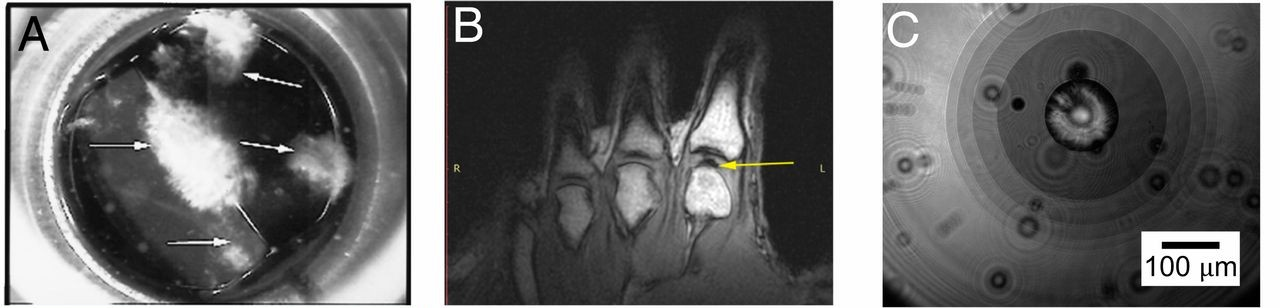
\includegraphics[width=\textwidth]{images/cavitation_example.jpeg}
    \caption{\centering (A) Пример кавитации после установки искусственного сердечного клапана~\cite{10.1114/1.231} (B) Пример кавитации при хрусте суставов~\cite{10.1371/journal.pone.0119470} (C) Пример кавитации в синтетическом силиконе при лазерной абляции~\cite{10.1073/pnas.1920168117}}
    \label{fig:cavitation_example}
\end{figure}

Кавитация представляет собой сложное физическое явление, проявляющееся в разнообразных формах в зависимости от механизмов инициирования, динамики развития пузырей и условий окружающей среды. 
Среди всего многообразия видов кавитации особый интерес представляет лазерно-индуцированная кавитация, которая отличается высокой степенью пространственной и временной локализации кавитационных процессов, благодаря чему данный метод находит применение в областях, требующих более точного контроля воздействия, таких как микрохирургия, лазерная литотрипсия и обработка материалов. 
В настоящем исследовании основное внимание уделено детальному анализу лазерно-индуцированной кавитации, рассмотрению которой далее будет посвящена отдельная подглава. 
В следующем разделе приведена систематизированная характеристика иных видов кавитации, что позволяет получить целостное представление о данном явлении и его практической значимости.

\vspace{0.5\baselineskip}
\subsubsection{Виды кавитации}
\vspace{0.5\baselineskip}

% Введение
Кавитация проявляется в различных формах, каждая из которых имеет свои отличительные особенности. 
Это многообразие обусловлено разными механизмами возникновения и условиями протекания процесса.
В зависимости от характера возбуждающего воздействия, параметров окружающей среды и других параметров системы, различают несколько видов кавитации, каждый из которых обладает своими особенностями формирования, коллапса пузыря и динамики его развития.
Различия в механизмах зарождения и условиях развития кавитации приводят к существенной разнице в динамике процесса.
Эти особенности определяют как потенциальные области практического применения кавитационных эффектов, так и возможные меры защиты от их разрушительного воздействия.

% Лазерная кавитация
Кавитация может быть инициирована посредством внешних воздейтсвий, так, например, лазерные импульсы обеспечивают точное создание кавитационных пузырей с заданными параметрами. 
При фокусировке излучения в жидкости происходит локальное поглощение энергии, приводящее к образованию ударных волн и паровых полостей. 
Особый интерес представляет динамика пузырей вблизи твердых поверхностей, где их коллапс сопровождается формированием высокоскоростных микроструй, способных вызывать эрозионные повреждения. 
Исследование этих процессов важно как для предотвращения разрушений в технических системах, так и для медицинских применений.

% Гидродинамическая кавитация
Кавитация может наблюдаться в гидродинамических потоках, где она вызывается локальным снижением давления ниже порога насыщения, например, таких как потоки через сопла Вентури, узкие каналы или вокруг крыльев и лопастей пропеллеров~\cite{10.1007/1-4020-2233-6}.
Когда скорость потока резко возрастает, статическое давление в соответствии с уравнением Бернулли~\ref{eq:bernulli} падает

\vspace{1em}
\begin{equation}
    \displaystyle {\frac {\rho v^{2}}{2}}+\rho gh+p={\text{const}}
    \label{eq:bernulli}
\end{equation}
\vspace{1em}

Это приводит к образованию кавитационных пузырей, заполненных паром и газами, растворенными в жидкости.
Формирование пузырей начинается с появления зародышевых полостей (кавитационных ядер), которыми могут служить микроскопические газовые включения или неоднородности на твердых поверхностях. 
При достижении критического перепада давления пузыри быстро расширяются, а затем коллапсируют при попадании в зону с более высоким давлением. 
Коллапс сопровождается ударными волнами, локальным нагревом.
Среди факторов, влияющих на динамику гидродинамической кавитации ключевыми являются: геометрия потока, влияющая на изменение скорости и, следовательно, давления потока, физические свойства жидкости, определяющие устойчивость пузырей, гидродинамические параметры, определяющие динамику движения потока.
Определение этих параметров позволяет прогнозировать кавитационные процессы, минимизировать их разрушительное воздействие и использовать их в полезных приложениях.

% Акустическая кавитация
В то же время кавитация может происходить в статичной или почти статичной жидкости.
При воздействии осциллирующего давления на свободную поверхность жидкости в резервуаре могут возникать кавитационные пузырьки, если амплитуда осцилляции достаточно велика.
Такой тип кавитации называется акустической.
Акустическая кавитация представляет собой процесс образования и последующего интенсивного схлопывания пузырьков в жидкости под воздействием акустических волн высокой интенсивности. Акустические волны, являющиеся распространением колебаний давления со скоростью звука в средах, таких как жидкости, газы или твердые тела, способны создавать циклические изменения давления, что является ключевым механизмом в развитии данного явления. 
При воздействии ультразвуковых волн в жидкости, возникают крошечные пузырьки газа, которые в фазе разрежения ультразвуковой волны увеличиваются в размерах из-за снижения давления, а затем быстро сжимаются при переходе в фазу сжатия. 
Если амплитуда акустического давления достаточна, пузырьки асимметрично коллапсируют, формируя микроструи жидкости.
В многопузырьковых системах взаимодействие между пузырями приводит к образованию кластеров, что усложняет динамику процесса из-за переизлучения ударных волн и экранирования акустического поля.
Помимо общих параметров кавитации, на процесс акустической кавитации также влияют параметры акустических колебаний, такие как частота и амплитуда, например, при увеличении частоты, уменьшается максимальный размер пузырьков перед коллапсом, но увеличивается интенсивность локального нагрева и испускаемых ударных волн~\cite{10.1007/1-4020-2233-6}.

% Игольная кавитация
Кавитация, индуцированная воздействием иглы, представляет собой процесс, включающий два последовательных этапа: первый — это прокол исследуемого образца при помощи иглы, а второй — создание локального давления в жидкости на кончике иглы до тех пор, пока при достижении критического уровня давления не произойдёт резкая деформация образца. 
Образование кавитационного пузыря в данном случае связано с быстрой деформацией жидкости или мягкого материала под действием механического импульса, создаваемого кончиком иглы. 
При этом давление в ограниченном объёме может быстро падать до значений ниже давления насыщенных паров, что инициирует фазовый переход и образование пузыря. 
Как и в случае с другими видами кавитации, важную роль играет скорость распространения давления, а также инерционные характеристики окружающей среды.
Малый объём зоны воздействия, пропорциональный \(r^3\), и высокая манёвренность иглы делают этот метод точным инструментом для локального анализа с возможностью прецизионного управления положением. 
Ключевым преимуществом метода является его способность оценивать механические свойства материалов на различных масштабах, начиная от микроскопического уровня. 
Однако использование данного подхода может быть осложнено при анализе материалов, размеры которых сопоставимы с характерными дефектами или гетерогенностями, присутствующими в структуре. 
Кроме того, значительную роль играют условия нагружения, которые могут быть заданы в форме фиксированного давления или фиксированного объёма. 
Для анализа жёстких материалов, которые затруднительно изучать при использовании методов с контролем давления, предпочтительно применять условия с фиксированным объёмом, что позволяет оптимизировать исследование под специфические свойства таких материалов~\cite{10.1039/c5sm00230c, 10.1039/b909237d}.
Такой подход нашёл применение в области биомеханики, например, для измерения локальных модулей упругости биологических тканей, а также при тестировании гидрогелей, композитов и других мягких материалов.

% каскадная кавитация
Каскадная кавитация представляет собой явление, при котором образование одного кавитационного пузыря приводит к формированию последующих пузырей, создавая цепную реакцию кавитационных событий.
В отличие от одиночных пузырей, возникающих в результате единичного воздействия, каскадная кавитация характеризуется многоступенчатым процессом, при котором каждый коллапс пузыря может инициировать образование новых пузырей за счёт высвобождающейся энергии и возникающих ударных волн.
Механизм каскадной кавитации основан на нелинейных взаимодействиях между пузырями и средой. 
При коллапсе пузыря генерируются высокоэнергетические ударные волны и струйные потоки, способные снизить локальное давление в прилегающих участках жидкости. 
Это, в свою очередь, может инициировать образование новых пузырей, особенно в областях, где уже имеются микроскопические неоднородности или газовые включения. 
Процесс может повторяться многократно, переходя в автокаталитическую форму, в которой каждый новый пузырь способствует созданию следующего.
Основными параметрами, определяющими поведение каскадной кавитации, являются начальная энергия возбуждающего импульса, концентрация зародышей кавитации в жидкости, расстояние между пузырями, вязкость среды, а также характер распространения ударных волн. 
В высокоэнергетических системах каскад может развиваться особенно интенсивно, формируя плотные кластеры пузырей и вызывая сложные гидродинамические эффекты, включая турбулентность, локальное повышение температуры и кавитационное разрушение окружающего материала.
Каскадная кавитация играет важную роль в различных приложениях, где необходимо масштабное воздействие на материал или среду~\cite{10.1016/j.ultsonch.2025.107295, 10.1016/j.ultsonch.2004.01.006}.

\vspace{0.5\baselineskip}
\subsubsection{Применение кавитации}
\vspace{0.5\baselineskip}

Кавитация имеет широкий спектр практических приложений в различных сферах и наиболее часто встречается в промышленном оборудовании и медицине.

Литотрипсия — это метод терапии, основанный на фокусировке ударных волн на целевом участке внутри тела с целью дистанционного разрушения камней в почках или желчном пузыре. Для повышения эффективности процедуры пациента помещают в водную ванну, чтобы акустическое сопротивление среды максимально соответствовало сопротивлению тела. Ударные волны направляются на область расположения камня, после чего производится серия импульсов, чтобы раздробить камень на фрагменты, которые организм сможет вывести естественным образом. 
Роль кавитации в процессе разрушения камня может варьироваться: в зависимости от подбора параметров она может как способствовать разрушению, так и стать причиной значительных повреждений окружающих тканей.~\cite{10.1134/1.1591291, 10.1016/0301-5629(87)90076-7, 10.1016/s0140-6736(80)92335-1}

Кавитационная обработка поверхности (пининг) представляет собой процесс улучшения свойств материалов за счёт воздействия, возникающего при схлопывании кавитационных пузырьков. 
В результате этого воздействия на поверхности материала формируется пластическая деформация и остаточные сжимающие напряжения, что улучшает прочностные характеристики и усталостную стойкость материала. 
В отличие от традиционного дробеструйного упрочнения, кавитационный пининг вызывает меньшее увеличение шероховатости поверхности благодаря отсутствию механических столкновений твёрдых частиц, а обработка проводится в пределах инкубационного периода кавитации, исключая эрозионные повреждения.~\cite{10.3390/app13116702, 10.3390/met10020270}

\begin{figure}[h]
    \centering
    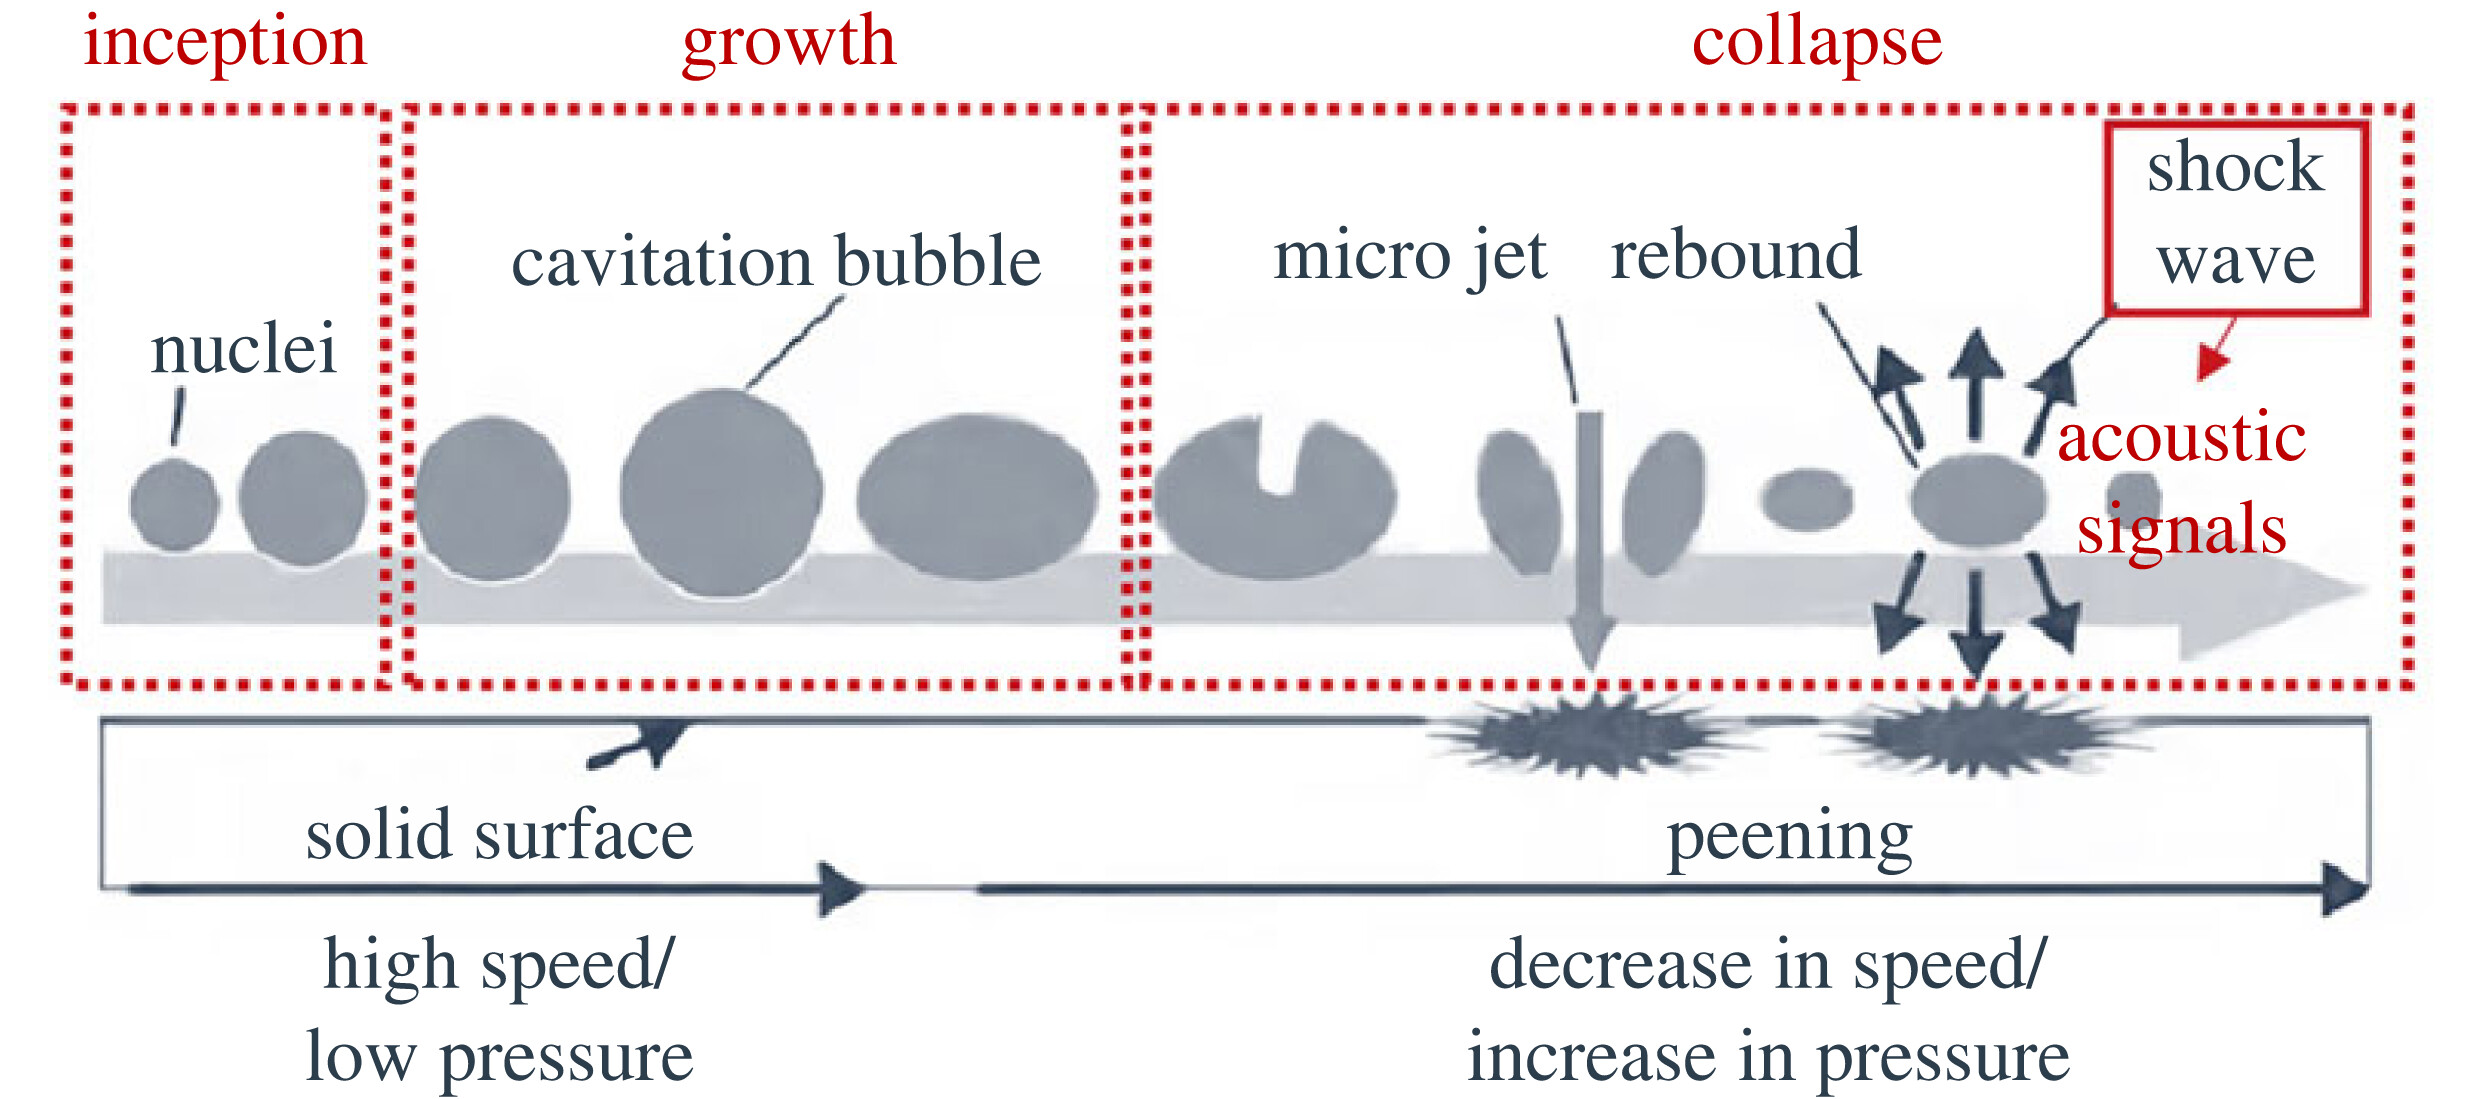
\includegraphics[width=\textwidth]{images/peening_scheme.jpg}
    \caption{\centering Схематичное изображение процесса кавитационной обработки поверхности~\cite{10.1098/rsta.2022.0402}}
    \label{fig:peening}
\end{figure}

Кавитация в поточной системе возникает, когда статическое давление в любой точке потока падает ниже парциального давления жидкости при рабочей температуре. Возникающая кавитация приводит к образованию выщербин или эрозии поверхности, что в долгосрочной перспективе способно вызвать отказ компонентов. Возникновение кавитации может отрицательно повлиять на работу оборудования задолго до выхода его из строя (рисунок~\ref{fig:erosion}). Поэтому конструкторы прилагают особые усилия, чтобы проектировать оборудование таким образом, чтобы избежать кавитации в ожидаемом диапазоне эксплуатации. Однако в случае сложных и капиталоемких инженерных систем, таких как ядерный реактор, не всегда возможно полностью избежать кавитации в процессе нормальной эксплуатации из экономических соображений.~\cite{10.1016/j.wear.2016.12.009}

\begin{figure}[h]
    \centering
    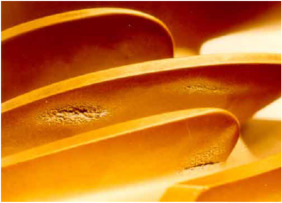
\includegraphics[height=.25\textheight]{images/erosion.png}
    \caption{\centering Кавитационное повреждение рабочего колеса смешанного насоса~\cite{10.1016/j.wear.2016.12.009}}
    \label{fig:erosion}
\end{figure}



Акустическая кавитация находит широкое применение в различных отраслях. 
В пищевой промышленности она используется для ускорения процессов смешивания и экстракции, в энергетике — для очистки поверхностей и обработки материалов, а в нанотехнологиях — для синтеза наночастиц. 
В медицине акустическая кавитация активно применяется в терапевтических и диагностических целях. Фокусированная акустическая энергия способна изменять проницаемость биологических тканей, что способствует доставке лекарственных препаратов и генетического материала в клетки, особенно при лечении онкологических заболеваний. 
Коллапсирующие пузырьки играют ключевую роль в повышении эффективности доставки и проникновения.
Высокоинтенсивный фокусированный ультразвук также успешно применяется в таких процедурах, как удаление предопухолевых тканей и литотрипсия, где контролируемая кавитация повышает эффективность и скорость лечения.
Несмотря на широкий спектр применений, реологические аспекты акустической кавитации остаются недостаточно изученными. 
В отличие от лазерно-индуцированной кавитации, при которой возможно детальное исследование отдельных пузырьков, в акустической кавитации формируется облако микропузырьков. 
Это усложняет анализ их индивидуальной динамики, и поэтому исследования преимущественно сосредоточены на коллективных характеристиках облака, таких как пороговое давление и общая стабильность. 
Современные экспериментальные методики, направленные на точное описание динамики кавитационных пузырьков, продолжают способствовать углублению знаний о физических процессах, сопровождающих акустическую кавитацию~\cite{10.1007/978-3-319-68237-2_1, 10.1016/b978-0-12-801530-8.00003-7, 10.1081/asr-200030202, 10.1016/j.ultsonch.2010.11.016}.

Одним из наиболее современных и интересных методов применения кавитации, является адресная доставка лекарств с использованием искусственных центров кавитации, активирующихся при помощи ультразвука.
Искусственное создание центров кавитации открывает новые возможности в медицинских технологиях. 
В последние годы активно развиваются методы направленного введения кавитационных ядер в целевую область, что позволяет значительно повысить контролируемость терапевтических процедур. 
Особенно перспективно это направление в HIFU-терапии (фокусированный ультразвук высокой интенсивности), где предварительное введение кавитационных центров обеспечивает более точное воздействие и снижает повреждение окружающих тканей.
Наиболее ярким примером этой технологии стало применение липосом и специальных микропузырьков в сочетании с фокусированным ультразвуком. 
Липосомы - наноразмерные сферические структуры (до 10 мкм) из фосфолипидов, аналогичных клеточным мембранам. 
Их уникальность заключается в возможности точной настройки структуры и содержимого, избирательного прикрепления к определенным клеткам и переноса газообразной внутренней части, реагирующей (взрывающейся) при воздействии ультразвука~\ref{fig:cancer}.
Это легло в основу инновационного метода - сонопорации, где ультразвуковая активация доставляет лекарственные вещества непосредственно в целевые клетки~\cite{10.1136/bmj.322.7296.1222}. 
Такие технологии создают принципиально новые возможности для точной доставки химиотерапевтических препаратов, локального воздействия на патологические очаги, минимизации системных побочных эффектов~\cite{10.2147/dddt.s31564}.


\begin{figure}[H]
    \centering
    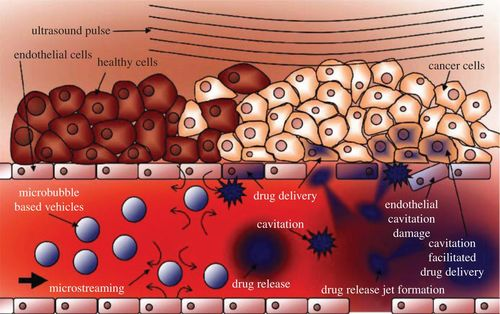
\includegraphics[width=.9\textwidth]{images/cancer.png}
    \caption{\centering Схема лечения рака липосомами и ультразвуком~\cite{10.2147/dddt.s31564}}
    \label{fig:cancer}
\end{figure}



Гидродинамическая кавитация изначально рассматривалась как перспективная альтернатива ультразвуковой кавитации в процессах передовой окислительной обработки благодаря её потенциальной энергоэффективности и возможности масштабирования для промышленных применений. Основной механизм гидродинамической кавитации заключается в образовании, росте и последующем схлопывании пузырьков под воздействием колебаний давления, что сопровождается локальными пиками температуры и давления, приводящими к инициации химических реакций.
Изучение процессов гидродинамической кавитации может быть проведено как на уровне индивидуальных пузырьков, так и на уровне их коллективного взаимодействия, что более характерно для высокоплотных кавитационных облаков. Эффективность кавитации определяется рядом ключевых параметров, включая количество пузырьков, их размеры и максимальные температуры, достигаемые при схлопывании. Эти характеристики могут быть исследованы экспериментально с использованием методов, таких как сонолюминесценция или анализ продуктов химических реакций, а также теоретически с применением методов компьютерного моделирования.~\cite{10.1016/j.ultsonch.2007.03.00}
Химическая активность системы существенно зависит от пространственного распределения пузырьков и условий, в которых протекают реакции. Оптимизация процессов гидродинамической кавитации требует выбора наиболее подходящего типа кавитации для заданной реакции, а также точного определения местоположения, где достигаются максимальная эффективность и энергия. Это позволяет установить связь между параметрами процесса и экспериментальными результатами, что является важным шагом для разработки теоретической основы и дальнейшей оптимизации технологий гидродинамической кавитации.~\cite{10.1016/j.crhy.2006.10.015}

Гидродинамическая кавитация представляет собой перспективную технологию обеззараживания воды, позволяющую эффективно уничтожать патогенные микроорганизмы без использования химических реагентов. 
В основе метода лежит способность кавитационных пузырей при схлопывании создавать экстремальные условия (давление до 1000 бар, локальный нагрев до 5000 К) и генерировать активные окислители, такие как гидроксильные радикалы. 
Эти факторы оказывают комплексное разрушающее действие на бактерии, вирусы и микроскопические водоросли. 
Комбинация гидродинамической кавитации с традиционными методами дезинфекции могут позволить достичь существенного снижения стоимости обработки. 
Современные исследования подтверждают экономическую целесообразность технологии даже в промышленных масштабах, однако для ее широкого внедрения требуется дальнейшая оптимизация конструкций реакторов и углубленное изучение механизмов воздействия на различные типы микроорганизмов~\cite{10.1016/j.scitotenv.2020.139606}.

\begin{figure}[h]
    \centering
    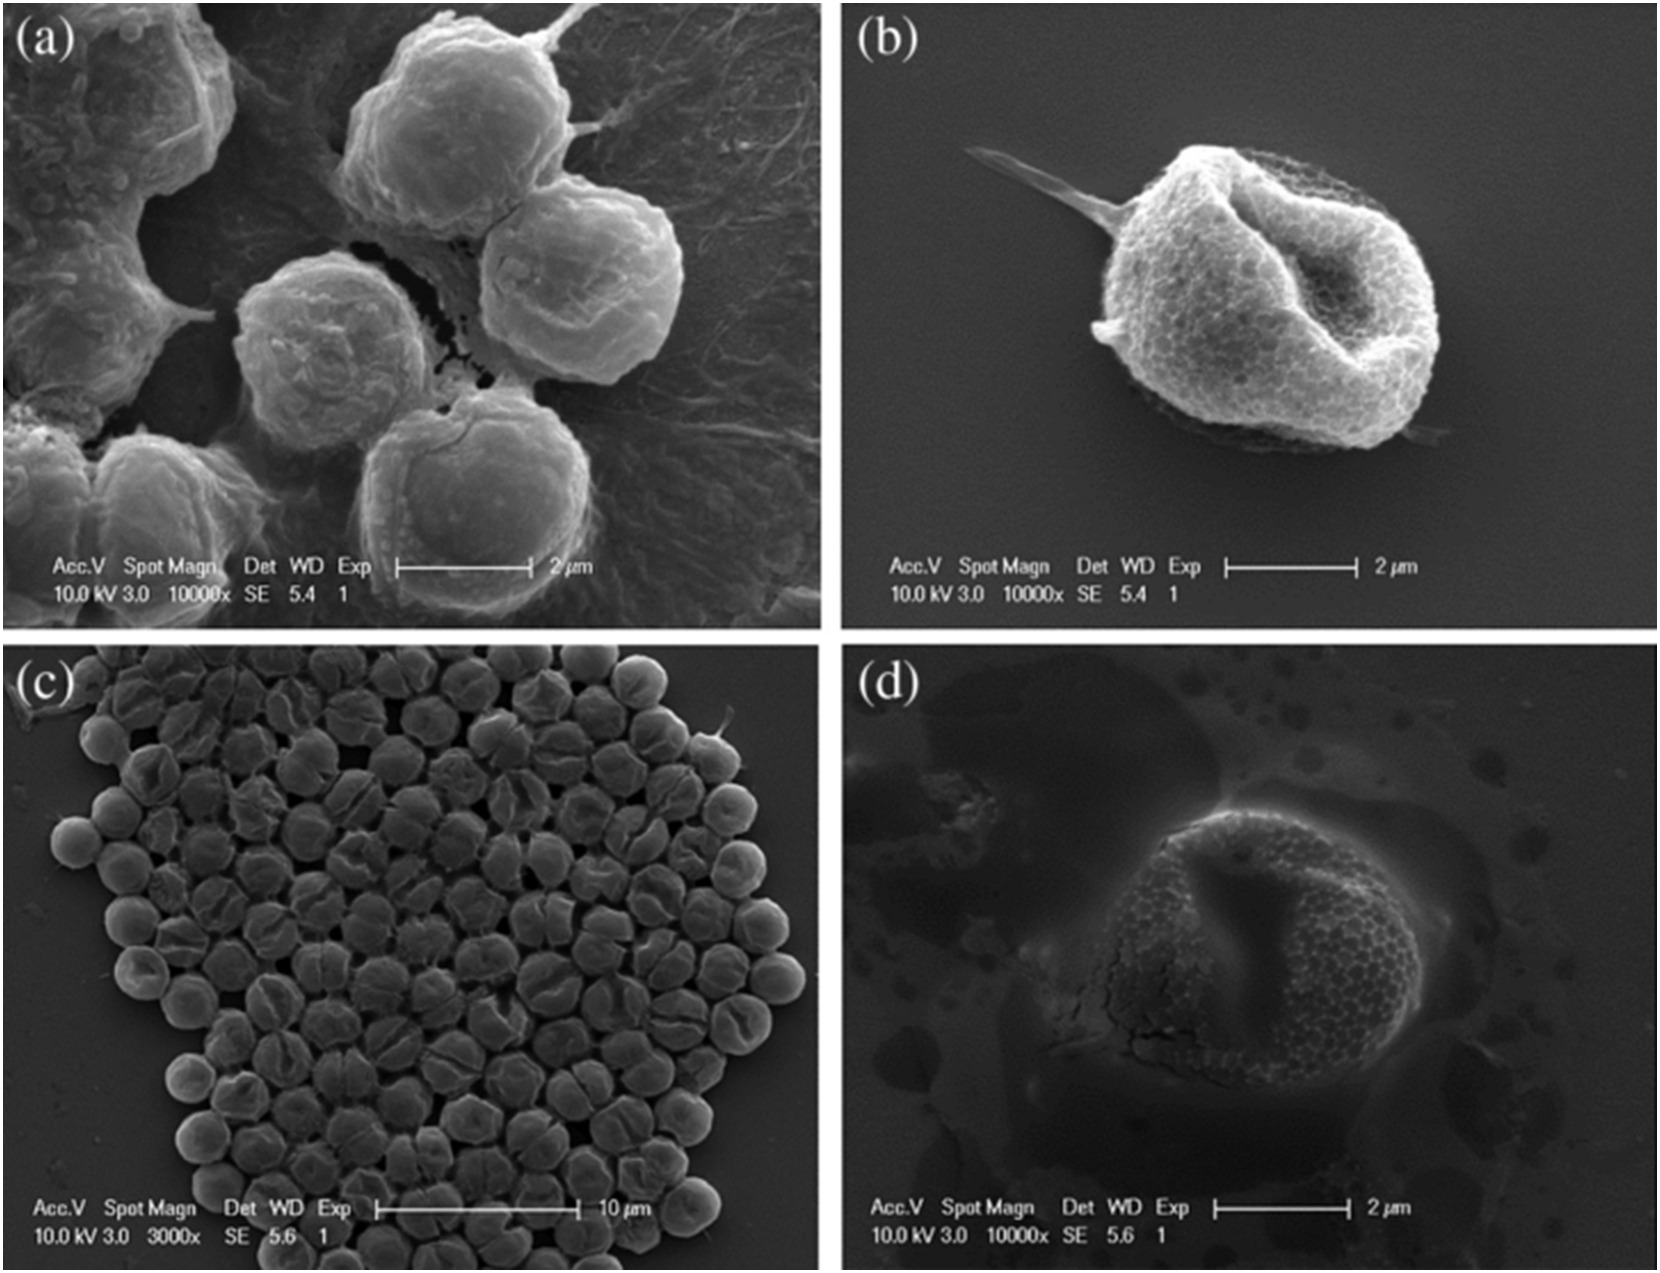
\includegraphics[height=.3\textheight]{images/desinfection.png}
    \caption{\centering Стереосканированные электронные микрофотографии клеток Microcystis aeruginosa после обработки с помощью гидродинамической кавитации  в течение (a) 0 мин, (b) 10 мин, (c) 30 мин и (d) 60 мин~\cite{10.1016/j.watres.2014.05.052}}
    \label{fig:desinfection}
\end{figure}


Другие методы кавитации демонстрируют ограниченные возможности в плане динамического и позиционного контроля, что значительно усложняет их использование для целенаправленных и управляемых исследований.

Одним из таких методов является кавитация, возникающая при воздействии ударных волн на интерфейсы в средах, таких как вода или биологические ткани. В данном случае формирование пузырей происходит вследствие воздействия чередующихся циклов давления и растяжения, индуцированных ударной волной. Пузырьки, образующиеся в процессе, быстро увеличиваются в размерах и затем коллапсируют, излучая вторичные сферические ударные волны. Эти волны, в свою очередь, взаимодействуют с ближайшей поверхностью облака пузырей, создавая на каждом этапе новый слой пузырьков. Методы генерации кавитации с использованием ударных волн включают применение таких установок, как устройства для падения капель, стержни Хопкинсона или системы, основанные на контролируемых взрывах.\cite{10.1073/pnas.1920168117}

Другим примером является кавитация, возникающая в образцах со сложной геометрией, где несжимаемость материала и наличие ограничивающих границ способствуют созданию высоких гидростатических давлений под действием внешнего механического напряжения. Подобный механизм кавитации можно наблюдать, например, при «хрусте» суставов. Контролируемое воспроизведение таких событий возможно посредством осевого сжатия коротких цилиндрических дисков, зафиксированных между двумя жесткими пластинами. Этот метод стал основой для первых наблюдений кавитации в мягких твердых материалах, что открывает новые перспективы для изучения данного явления в контексте моделирования динамики кавитационных пузырей.~\cite{10.1073/pnas.1920168117}


\vspace{0.5\baselineskip}
\subsection{Лазероиндуцированная кавитация}
\vspace{0.5\baselineskip}

Данное исследование сосредоточено на лазерно-индуцированной кавитации, которая обладает высокой точностью по сравнению с традиционными методами. 
Использование лазерных импульсов позволяет создавать локализованные кавитационные пузыри с заранее контролируемыми размерами и свойствами. 
В этом процессе высокоэнергетические лазерные импульсы фокусируются в определённой точке в жидкости, что приводит к генерации как ударных волн, так и паровых пузырей. 
Динамика этих пузырей, особенно их взаимодействие с твёрдыми поверхностями, имеет критическое значение для понимания их полезных и потенциально вредных эффектов. 
Например, коллапс кавитационного пузыря, расположенного вблизи твёрдой поверхности, может вызвать образование высокоскоростных струй, направленных на эту поверхность, что в свою очередь может привести к эрозионным повреждениям. 
Изучение поведения пузырей при различных условиях является важным аспектом для минимизации потенциальных повреждений в промышленных приложениях и повышения эффективности лазерных методов в медицинской практике.

Кавитация, индуцированная лазерным излучением, основывается на фокусированном поглощении оптической энергии, которое вызывает диэлектрический пробой в прозрачной среде и приводит к быстрому расширению полости. 
При традиционном подходе лазерный импульс высокой интенсивности инициирует ионизацию молекул среды, что усиливает её оптическое поглощение и вызывает лавинный процесс. 
Это приводит к резкому повышению температуры в локальной области и образованию кавитационного пузыря в течение наносекунд.~\cite{10.1007/s00339-010-6056-7}
Скорость расширения пузырька может достигать от 100 до 3000 м/с. Однако такая техника отличается высокой чувствительностью к локальным вариациям оптических и физических свойств материала, что снижает предсказуемость процессов в гетерогенных средах, таких как биологические ткани.
Альтернативный подход предполагает введение в исследуемую среду частиц, которые активно поглощают лазерное излучение. 
Этот метод устраняет необходимость диэлектрического пробоя и позволяет проводить процесс в более контролируемых условиях. 
Такая технология, называемая кавитацией с добавлением поглощающих частиц, снижает зависимость от оптической однородности среды, делая анализ динамики более количественным.


\begin{figure}[h]
    \centering
    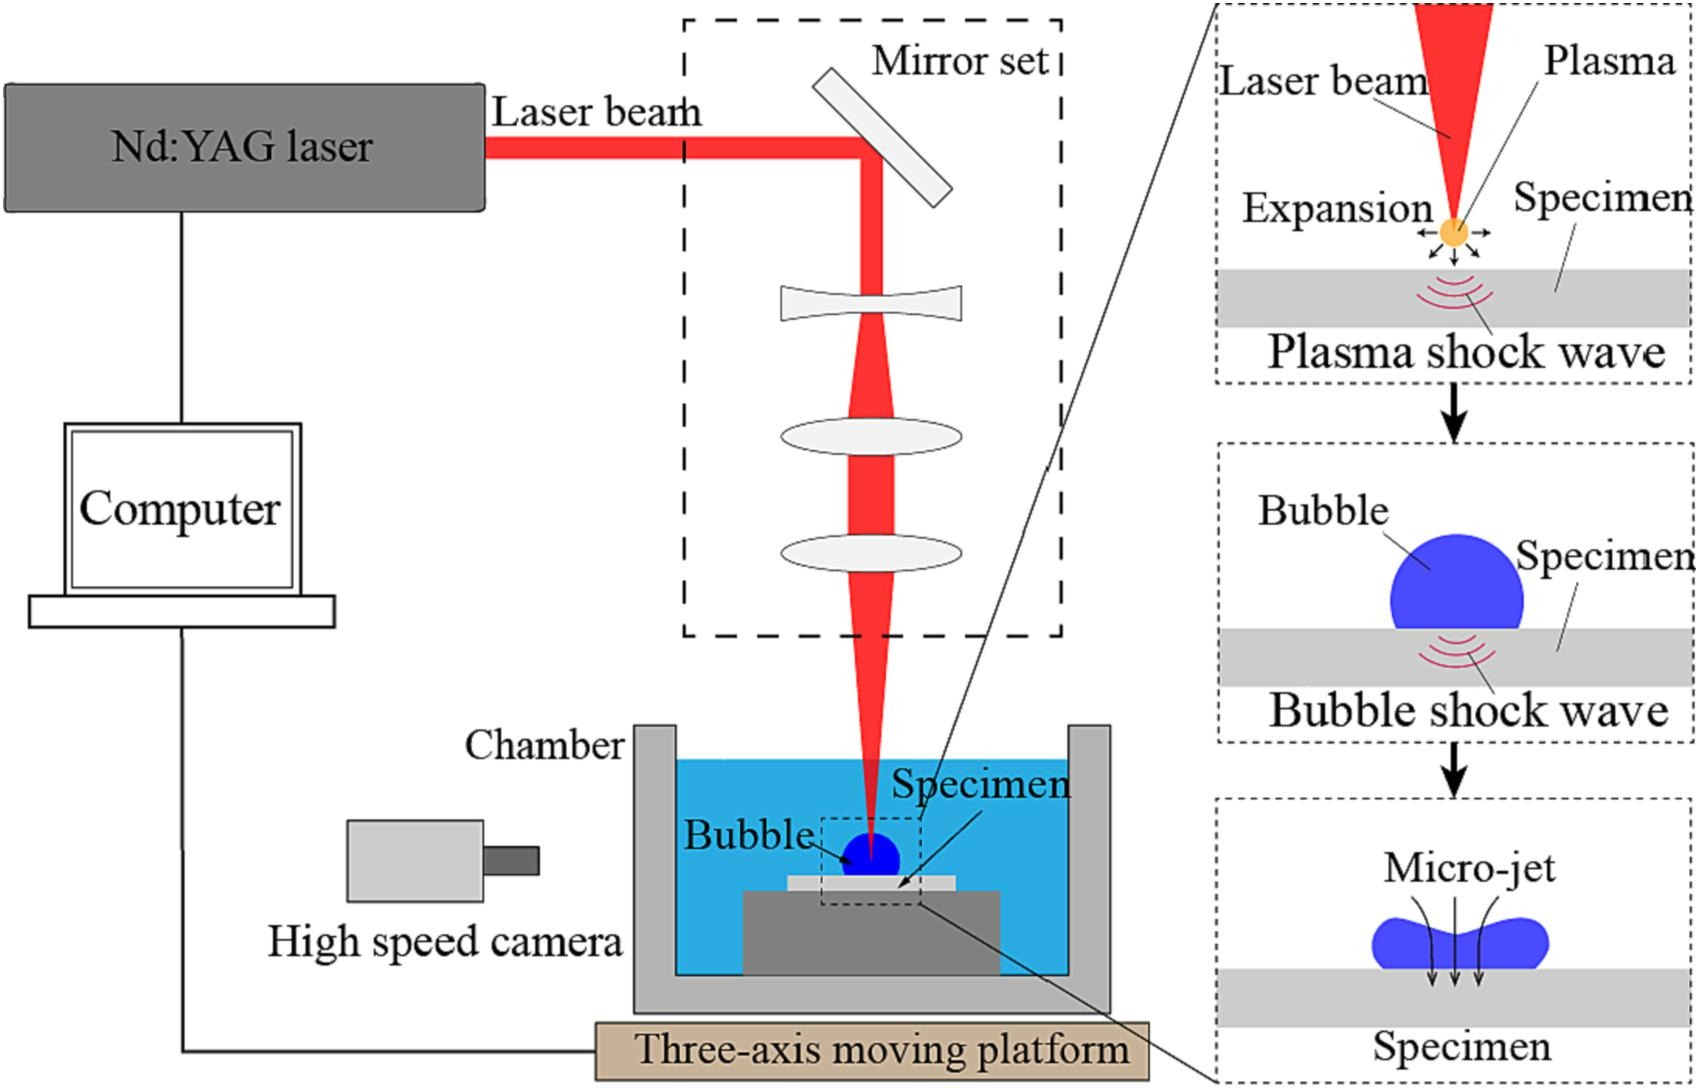
\includegraphics[height=.3\textheight]{images/laser_exp_scheme.jpg}
    \caption{\centering Схема экспериментальной установки для наблюдения лазероиндуцированной кавитации~\cite{10.1016/j.optlastec.2023.110212}}
    \label{fig:laser_exp_scheme}
\end{figure}

Принцип лазерной обработки поверхности с применением кавитации основывается на создании кавитационных пузырей в жидкости, которые воздействуют на поверхность материала при их схлопывании (рисунок~\ref{fig:laser_exp_scheme}).
Лазерный луч проходит через систему зеркал, фокусируется и направляется в жидкость, где возникает кавитационный пузырь. При схлопывании пузыря происходит воздействие на поверхность образца, вызывая пластическую деформацию и возникновение остаточного сжатия, что способствует улучшению прочностных характеристик материала и предотвращению роста трещин.

Процесс лазерной кавитации можно разделить на три основные стадии:
\begin{enumerate}
    \item Удар плазмы. Лазерный импульс поглощается водой вблизи фокуса, что приводит к её ионизации и образованию плазмы. Когда плотность мощности лазера превышает порог пробоя воды, плазма образуется мгновенно и наносит удар по поверхности материала.
    \item Схлопывание пузыря. После образования плазмы она расширяется, сжимая окружающую жидкость, что приводит к образованию кавитационного пузыря. В процессе расширения пузыря давление внутри него снижается, и когда оно становится ниже внешнего давления, пузырь схлопывается, генерируя ударную волну и водяной поток, которые дополнительно воздействуют на поверхность образца.
    \item Дополнительные пульсации. Пузырь может несколько раз расширяться и схлопываться, но из-за потери энергии на предыдущих этапах воздействия последующие удары становятся менее интенсивными и обычно не оказывают значительного влияния.
\end{enumerate}
Этот процесс способствует образованию пластической деформации и остаточного сжатия на поверхности материала, что в свою очередь улучшает его усталостную прочность и замедляет развитие трещин.~\cite{10.1016/j.optlastec.2023.110212}

% Применение
Лазерноиндуцированная кавитация имеет широкий спектр применений во многих областях, в частности в биомедицине, за счет простоты реализации, а также высокой точности и локализации явления.

Методы кавитации, индуцированной лазером, находят широкое применение в биомедицинских и инженерных задачах, таких как визуализация и терапия тканей, разрушение клеточных структур, доставка лекарственных препаратов, создание микроактуаторов и определение механических свойств материалов.~\cite{10.1364/ol.39.002599, 10.1063/1.3430989}
В случае работы с биологическими объектами, где оптическая неоднородность затрудняет прямое воздействие лазерного излучения, используют оптические волокна для обеспечения точной передачи энергии в заданную область, что особенно эффективно для изучения толстых тканевых образцов.
Динамика кавитационных процессов, индуцированных лазером, обычно развивается в временных масштабах от микросекунд до миллисекунд. Для наблюдения таких процессов в реальном времени применяют высокоскоростные камеры. Кроме того, для ультрабыстрого анализа используют освещение с высокой частотой повторения, например, фемтосекундные лазеры с системами выбора импульсов, что позволяет детально изучить этапы развития и коллапса пузырьков.~\cite{10.1016/j.jmps.2017.12.006}

Фокусированное лазерное излучение, известное как метод фотодеструкции, создает кавитационные пузыри, способные выполнять точные микроразрезы тканей. Эта технология, часто называемая «лазерным скальпелем», нашла широкое применение в неинвазивной офтальмологической хирургии, где импульсы Nd:YAG-лазера позволяют проводить точные внутриглазные операции~\cite{10.1007/bf00130696,10.1016/s0146-2776(80)80036-x, 10.1017/s0022112089002314, 10.1121/1.415878}.

Ключевым аспектом данной методики является использование повторяющихся низкоэнергетических импульсов, которые минимизируют зону термического повреждения. 
Как показали исследования Фогеля и др.~\cite{10.1017/s0022112089002314, 10.1121/1.415878}, степень повреждения ткани пропорциональна кубическому корню от энергии импульса, поэтому оптимальным решением становится применение импульсов минимальной энергии, достаточной для инициирования кавитации. 
Эксперименты подтвердили, что пикосекундные импульсы обеспечивают более контролируемое воздействие по сравнению с наносекундными. На рисунке~\ref{fig:laser_induced} представлены характерные изображения, демонстрирующие ударную волну от лазерного импульса и последующее образование кавитационного пузыря для двух типов лазеров.

Метод лазерной фотодеструкции также успешно применяется в других областях медицины, например, лазерной литотрипсии, где способствует успешному разрушению конкрементов в мочевыводящих путях~\cite{10.1089/end.2012.0217, 10.1364/boe.9.004552}

\begin{figure}[h]
    \centering
    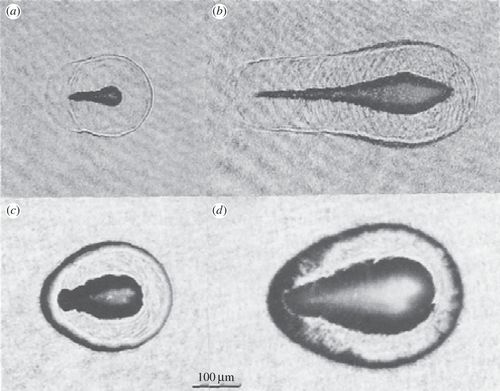
\includegraphics[height=.3\textheight]{images/laser_induced.png}
    \caption{\centering Пузырьки и ударные волны, формируемые в фокусе
пикосекундными лазерными импульсами (a,b) и
наносекундными импульсами (c,d)~\cite{10.1016/j.optlastec.2023.110212}}
    \label{fig:laser_induced}
\end{figure}

\vspace{0.5\baselineskip}
\subsection{Моделирование кавитации}
\vspace{0.5\baselineskip}

Впервые динамика кавитации и сферических пузырей была проанализирована Рэлеем в 1917 году~\cite{10.1080/14786440808635681, 10.1146/annurev.fl.09.010177.001045}. В модели предполагалось, что пузырь имеет сферическую форму, жидкость несжимаема, а внешнее давление остается постоянным. При этом эффекты поверхностного натяжения и вязкости жидкости были проигнорированы. На основе уравнения движения было показано, что радиус пузыря \( R(t) \) подчиняется следующему соотношению:

\vspace{1em}
\begin{equation*}
    R\ddot{R} + \frac{3}{2}\dot{R}^2 = \frac{p(R) - p_\infty}{\rho}
\end{equation*}
\vspace{1em}

\noindent где\quad \( \rho \) — плотность жидкости;

\( p_\infty \) — давление в жидкости вдали от пузырей;

\( p(R) \) — давление в жидкости на границе пузыря.

При этом \( p(R) \) также является давлением внутри пузыря.

Хотя модель Рэлея игнорировала вязкость жидкости и поверхностное натяжение, предполагая постоянное давление, эти эффекты можно учесть, расширив его динамическое уравнение. Плессе в 1949 году доработал уравнение Рэлея, включив в него влияние поверхностного натяжения и вязкости жидкости, но игнорируя сжимаемость жидкости, а также тепловые и массопереносные процессы ~\cite{10.1115/1.4009975}. Полученное уравнение стало известно как уравнение Рэлея-Плессе:

\vspace{1em}
\begin{equation*}
    R\ddot{R} + \frac{3}{2}\dot{R}^2 = \frac{1}{\rho} \left[ P_B - P_\infty - \frac{2\sigma}{R} - \frac{4\mu\dot{R}}{R} \right]
\end{equation*}
\vspace{1em}


Обе модели не учитывают сжимаемость жидкости. Однако, когда скорость движения стенки пузырька становится сопоставимой со скоростью звука в жидкости, учет сжимаемости становится необходимым. Гилмор рассмотрел сжимаемость и поверхностное натяжение жидкости, содержание и вязкость постоянного газа в пузырьке, при этом игнорируя процессы испарения, конденсации, диффузии газа через стенку пузырька и теплопроводности.~\cite{10.1115/1.4049933, 10.1017/cbo9781107338760} Модель Гилмора описывает движение пузырька следующим образом:

\vspace{1em}
\begin{equation*}
    \left( 1 - \frac{\dot{R}}{c} \right) R\ddot{R} + \frac{3}{2} \dot{R}^2 \left( 1 - \frac{\dot{R}}{3c} \right) = H \left( 1 + \frac{\dot{R}}{c} \right) + \frac{R\dot{H}}{c} \left( 1 - \frac{\dot{R}}{c} \right)
\end{equation*}
\vspace{1em}

\noindent где\quad \( R \) — радиус пузырька;

\( \dot{R} \) и \( \ddot{R} \) — первая и вторая производные радиуса по времени, представляющие скорость и ускорение стенки пузырька соответственно;

\( c \) — локальная скорость звука на стенке пузырька

\( H \) — разница энтальпий между интерфейсом пузырька и окружающей средой воды.

Фудзикава и Акаматсу~\cite{10.1017/s0022112080002662} провели численный анализ физического поведения пузырька во время его схлопывания в жидкости и разработали теоретическую модель. Принцип работы модели представлен на риснуке~\ref{fig:fujikawa_model}. Математическое уравнение учитывает такие факторы, как сжимаемость и вязкость жидкости, неравновесную конденсацию пара, теплопроводность и температурные скачки на фазовом интерфейсе. Численное решение процесса схлопывания пузырька определяется в момент, когда пузырёк достигает минимального радиуса, а волна давления распространяется наружу в жидкость. Результаты показали, что испарение и конденсация оказывают значительное влияние на динамическое поведение пузырьков. Модель также учитывает воздействие водяного пара и неконденсируемых газов на процесс схлопывания пузырька и распространение ударных волн.

\begin{figure}[h]
    \centering
    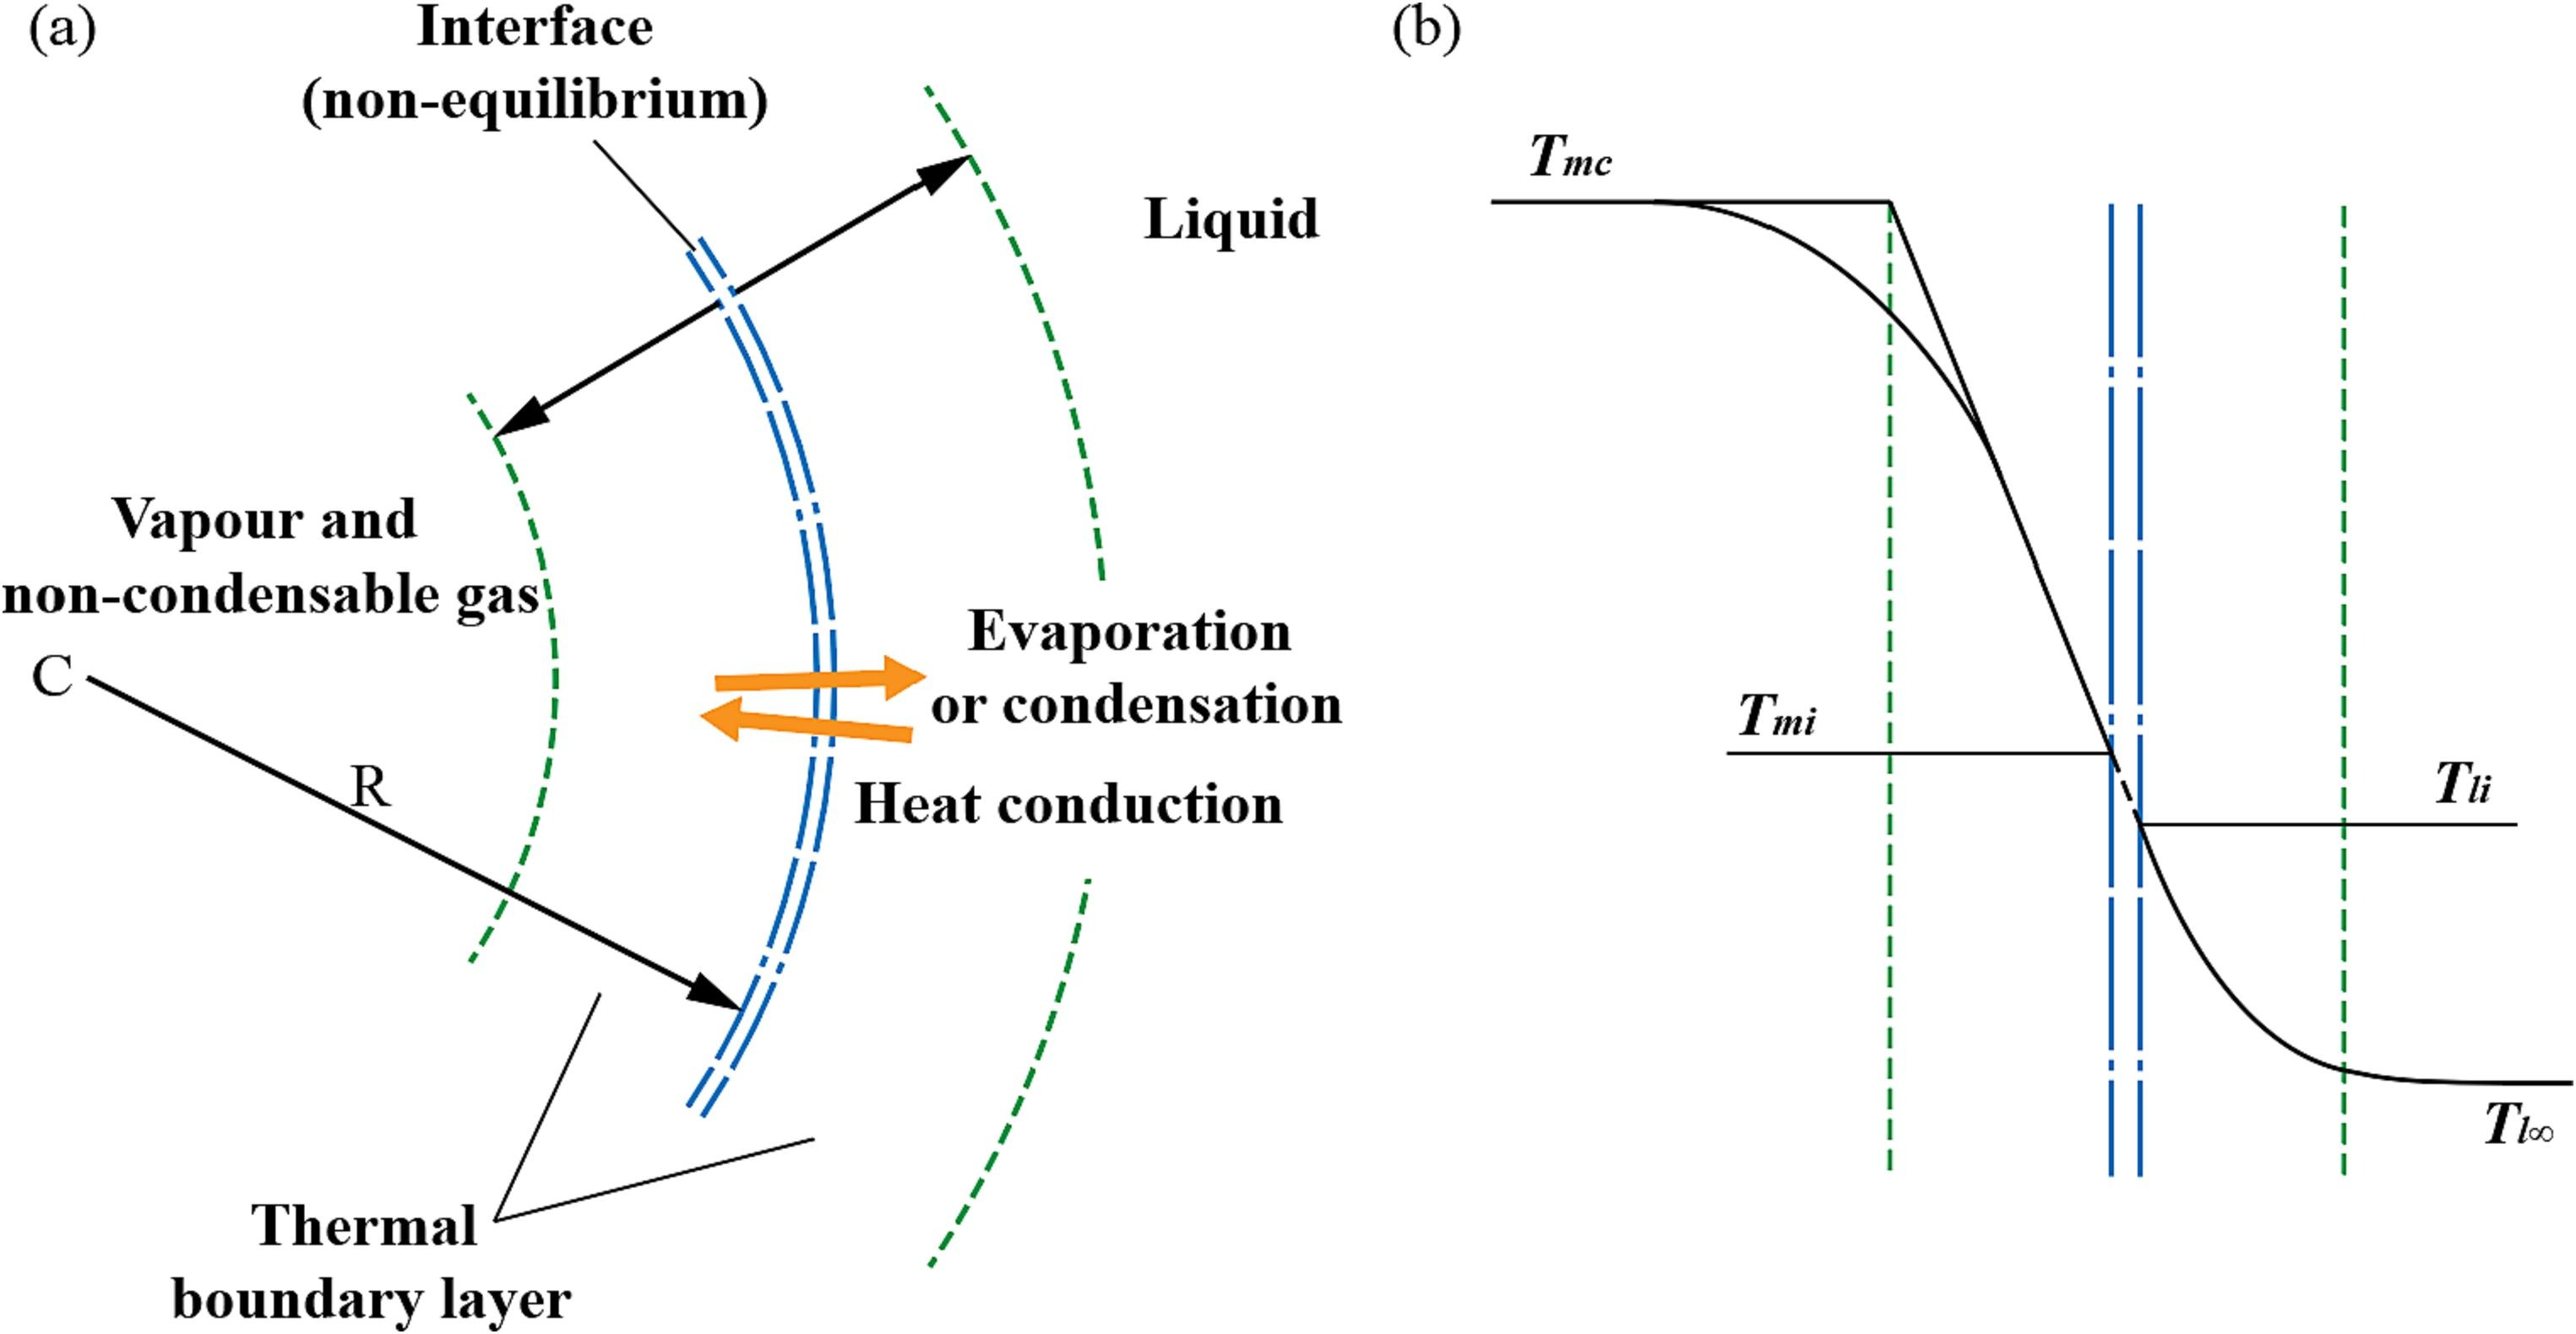
\includegraphics[height=.3\textheight]{images/fujikawa_model.jpg}
    \caption{\centering (а) схема модели; (б) распределение температуры внутри и снаружи пузырька}
    \label{fig:fujikawa_model}
\end{figure}

Ахатов и соавторы ~\cite{10.1063/1.1401810} разработали математическую модель симметричного движения сферических пузырьков, вызванного лазером. Модель учитывает сжимаемость пузырька и жидкости, тепловые и массовые переносы внутри пузырька и жидкости, а также неравновесные процессы испарения и конденсации на стенке пузырька. Поскольку взаимодействие воды и пара играет важную роль в динамике пузырьков, в модели используется подробный подход Герца-Кнудсена-Лангмюра для описания процессов испарения и конденсации. Модель учитывает возможность достижения и превышения критического состояния, при котором исчезают термодинамические различия между фазами. 
Дополнительно используется сложное уравнение состояния воды в форме Мие-Грюнайзена, подходящее для описания очень сильного сжатия и умеренного расширения воды. Предполагается, что пузырёк состоит преимущественно из водяного пара с небольшим количеством неконденсируемого газа. В модели присутствуют два свободных параметра: коэффициент, регулирующий испарение и конденсацию, и массовая концентрация неконденсируемого газа внутри пузырька. Модель начинает работать с момента, когда пузырёк достигает своего максимального радиуса \( R_{\text{max}} \).


\vspace{0.5\baselineskip}
\subsection{Цель и задачи работы}
\vspace{0.5\baselineskip}

В одной из серий экспериментальных исследований, выполненных в Институте общей физики РАН, изучалась система, включающая биологическую ткань и микросекундный лазер, формирующий импульс, направленный на образец ткани.
Характерной особенностью эксперимента являлся режим работы лазера, обеспечивающий создание серии лазерных импульсов, которая вызывала образование кавитационного пузыря сложной геометрической формы.
Эксперименты проводились как с одиночным лазерным импульсом, так и с каскадной серией из трёх импульсов. 
В результате были получены изображения, отражающие динамику формирования кавитационного пузыря в воде после лазерного воздействия на ткань.

\begin{figure}[h]
    \centering
    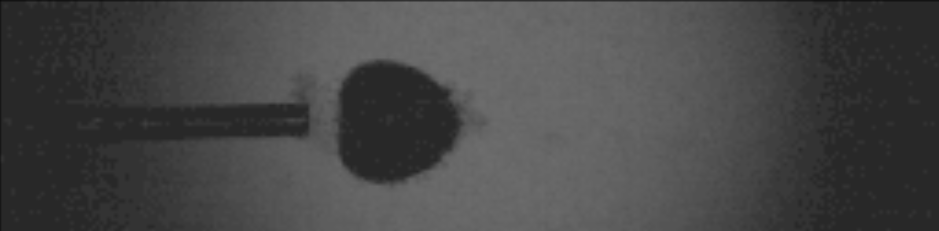
\includegraphics[width=\textwidth]{images/laser_exp_1.png}\\
    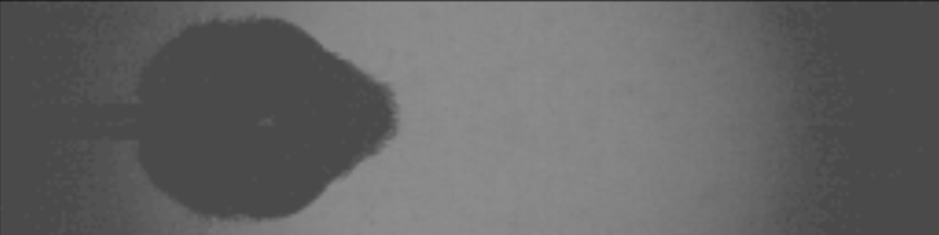
\includegraphics[width=\textwidth]{images/laser_exp_3.png}
    \caption{\centering Лазероиндуцированные кавитационные пузырьки с помощью
одиночного и тройного микросекундного лазерного импульса,
наблюдаемые в экспериментах}
    \label{fig:experiments}
\end{figure}


Для более подробного изучения полученной в результате эксперимента динамики кавитационного пузыря и его свойств были проведены компьютерные моделирования и сформулированы следующие цель и задачи настоящей работы.

\textbf{Цель работы} -- изучение динамики каскадного кавитационного пузыря, индуцированного лазерным излучением, методами компьютерного моделирования

\textbf{Задачи:}
\begin{itemize}
    \item Построение математической модели для изучения динамики кавитационного пузыря, индуцированного лазерным излучением
    \item Проведение систематических расчетов динамики кавитационного пузыря, индуцированного лазерным излучением, методами компьютерного моделирования
    \item Разработка алгоритмов постобработки
    \item Анализ результатов, построение распределений параметров динамики
\end{itemize}